\documentclass[tikz,border=6pt]{standalone}
\usepackage{tikz}
\usetikzlibrary{shapes,arrows.meta,positioning,calc,fit,backgrounds}
\usepackage{amsmath,amssymb}

\begin{document}
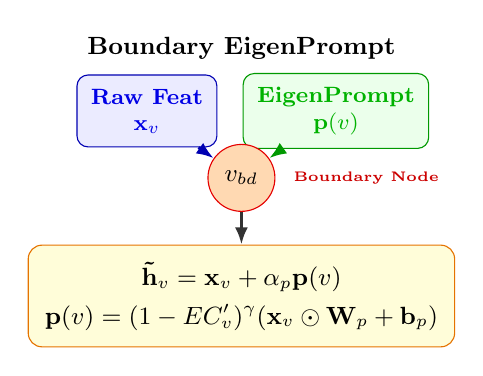
\begin{tikzpicture}[
    font=\sffamily\footnotesize,
    >=Latex,
    bound/.style={circle, draw=red!90!black, fill=orange!30, minimum size=8.5mm, inner sep=0pt, font=\bfseries\small},
    featbox/.style={draw=blue!70!black, fill=blue!8, rounded corners=4pt, inner sep=5pt, align=center, font=\bfseries\footnotesize, text=blue!90!black},
    promptbox/.style={draw=green!60!black, fill=green!8, rounded corners=4pt, inner sep=5pt, align=center, font=\bfseries\footnotesize, text=green!70!black},
    outbox/.style={draw=orange!90!black, fill=yellow!15, rounded corners=5pt, inner sep=6pt, align=center, font=\bfseries\small}
]

    % Header Title
    \node[font=\bfseries\small] at (1.2, 2.8) {Boundary EigenPrompt};

    % Inputs
    \node[featbox]   (raw) at (0.0, 2.0) {Raw Feat\\$\mathbf{x}_v$};
    \node[promptbox] (prm) at (2.4, 2.0) {EigenPrompt\\$\mathbf{p}(v)$};

    % Central Boundary Node
    \node[bound] (vbd) at (1.2, 1.15) {$v_{bd}$};
    \node[right=3pt of vbd, font=\tiny\bfseries, text=red!80!black] {Boundary Node};

    % Arrows to Boundary Node
    \draw[-{Latex[length=2.2mm]}, line width=1.1pt, blue!70!black] (raw) -- (vbd);
    \draw[-{Latex[length=2.2mm]}, line width=1.1pt, green!60!black] (prm) -- (vbd);

    % Output Mathematical Box
    \node[outbox] (out) at (1.2, -0.35) {
        $\mathbf{\tilde{h}}_v = \mathbf{x}_v + \alpha_p \mathbf{p}(v)$\\[3pt]
        $\mathbf{p}(v) = (1 - EC'_v)^\gamma (\mathbf{x}_v \odot \mathbf{W}_p + \mathbf{b}_p)$
    };

    % Arrow to Output
    \draw[-{Latex[length=2.2mm]}, line width=1.1pt, black!80] (vbd) -- (out);

\end{tikzpicture}
\end{document}
